% \documentclass{article}
% \usepackage[utf8]{inputenc}
% \usepackage{fullpage}
% \usepackage{setspace}
% \usepackage[hang,flushmargin]{footmisc} %control footnote indent
% \usepackage{url} % for website links
% \usepackage{amssymb,amsmath}%for matrix
% \usepackage{graphicx}%for figure
% \usepackage{appendix}%for appendix
% \usepackage{float}
% \floatstyle{plaintop}
% \restylefloat{table}
% \usepackage{multirow}
% \usepackage{longtable}
% \usepackage{morefloats}%in case there are too many float tables and figures
% \usepackage{caption}
% \usepackage{subcaption}
% \usepackage{listings}
% \captionsetup[subtable]{font=normal}
% \usepackage{color}
% \usepackage{hyperref}
% \usepackage[round]{natbib}
% \usepackage{rotating} % rotate table by some degree
% \usepackage{rotfloat}



% %\usepackage{Sweave}
% \setlength{\parindent}{0em}
% \setlength{\parskip}{0.5em}


% \graphicspath{{0.plots/}}



% \begin{document}

%%%%%%%%%%%%%%%%%%%%%%%%%%%%%%%%%%%%
\section{Plan for Simulation Studies} 
%%%%%%%%%%%%%%%%%%%%%%%%%%%%%%%%%%%%
Simulation studies are designed mainly for two aims. First, to check the validity of our proposed fully Bayesian algorithm in estimating the regression coefficients in the new JM framework. Our focus of the simulation results lies on the accuracy (i.e. bias) and the precision (i.e. standard deviation) of our estimations based on the posterior distributions. The second simulation study is planned to check the performance of our proposed estimator of the survival probability given in (\ref{eqn:sample_mean}). This can be done by comparing our estimates with the ``gold standard'', which is calculated based on the true (simulated) value of random effects, fixed effects as well as the parameters.


%%%%%%%%%%%%%%%%%%%%%%%%%%%%%%%%%%%%
\subsection{Simulation Study 1 (Estimation Accuracy) }
%%%%%%%%%%%%%%%%%%%%%%%%%%%%%%%%%%%%
% \begin{equation}\label{eqn:joint}
% \left\{
% \begin{array}{l}
% y_{it} = \boldsymbol{\beta}^{\top}{\boldsymbol X}_{it} + \boldsymbol{\delta}^{\top}{\boldsymbol H}_{it} + {\boldsymbol u}_i^{\top}{\boldsymbol Z}_{it} + \varepsilon_{it} =\overset{\sim}{\tau}_{it} + \varepsilon_{it}\\
% h(T_i|\mathcal{T}_{iT_i}, {\boldsymbol W}_i;  \boldsymbol{\gamma}, \alpha_1, 
% \alpha_2) = h_0(T_i)\exp(\boldsymbol{\gamma}^{\top}{\boldsymbol W}_i + \alpha_1\boldsymbol{\delta}^{\top}{\boldsymbol H}_{iT_i} + \alpha_2{\boldsymbol u}_i^{\top}{\boldsymbol Z}_{iT_i})
% \end{array}
% \right.
% \end{equation}


The first simulation study is designed to to check the accuracy of our proposed fully Bayesian estimating algorithm, which is the crucial basis for future prediction performance. Following \cite{Alessio2014qrjm}, by varying the values of the association parameters $\alpha_1$ and $\alpha_2$ in our model (\ref{eqn:joint}), we will have four different settings for simulation study, which are:

\begin{enumerate}
\item $(\alpha_1, \alpha_2)=(0, 0)$, the two models are indepdent with each other
\item $(\alpha_1, \alpha_2)=(1, 0)$, the two models are related only through the observed heterogeneity in some covarites, i.e. ${\boldsymbol H}_{it}$ in our model
\item $(\alpha_1, \alpha_2)=(0, 1)$, the two models are related only through the unobserved heterogeneity, i.e. the random effects
\item $(\alpha_1, \alpha_2)=(1, 1)$, the depdence of the two models is explained by both observed and unobserved heterogeneity
\end{enumerate}


% In model (\ref{eqn:joint}) note that we have specific covariates ${\boldsymbol X}_{it}$ only for the longitudinal model and covariates ${\boldsymbol W}_{it}$ only for the survival model.


Under different combinations of $\alpha_1$ and $\alpha_2$ values, we choose the regression coefficients $\boldsymbol{\beta, \delta, \gamma}=(1, 1)^{\top}$, the covriates ${\boldsymbol Z}_{it}=(1, t)^{\top},\hspace{0.5em} {\boldsymbol H}_{it}=(h_{i1}, h_{i2}*t)^{\top},\hspace{0.5em} {\boldsymbol X}_{it}=(1, x_i)^{\top},\mbox{ and }\hspace{0.5em} {\boldsymbol W}_{i}=(w_{i1}, w_{i2})^{\top}$ with $h_{i1}, h_{i2}, x_i, w_{i1}$ and $w_{i2}$ generated from independent standard normal distributions, and the random effects  $\boldsymbol{u}_i$ from bivariate normal with mean 0, standard deviations equal 0.3 and correlation 0.16. We also fix $\sigma=1$ and vary the quantile $\tau$ among $\{0.25, 0.5, 0.75\}$ for the ALD specification when simulating longitudinal data.

To simulate the survival time data, for simplicity, we fix $h_0(s)=1$ and obtain the survival distribution as 

\[S(t|\boldsymbol{u}_i, {\boldsymbol H}_{it}, {\boldsymbol W}_i)=\exp\left\{-\frac{e^{\alpha_1(\delta_1H_{i1}+\delta_2H_{i2t}) + \alpha_2(u_{i1}+u_{i2}t) + \boldsymbol{\gamma}^{\top}\boldsymbol{W}_i} - e^{\alpha_1\delta_1H_{i1}+\alpha_2u_{i1} + \boldsymbol{\gamma}^{\top}\boldsymbol{W}_i}}{\alpha_2u_{i2}+\alpha_1\delta_2h_{i2}}\right\}\] when $\alpha_1\ne0$ or $\alpha_2\ne0$ and 

\[S(t|\boldsymbol{u}_i, {\boldsymbol H}_{it}, {\boldsymbol W}_i) =  \exp\{-te^{\boldsymbol{\gamma}^{\top}\boldsymbol{W}_i}\}\]
when $\alpha_1=\alpha_2=0.$ We then can obtain event time $T_i$ by inverting above survival function after generating $n$ random variates from standard uniform distribution. To obtain a censoring proportion around 25\%, we choose the censoring time $C_i/5$ be distributed according to $beta(4,1)$ . \par

To simulate the longitudinal data, we draw them independently from the ALD for the $\tau$th quantile, centered on 
\[\boldsymbol{\beta}^{\top}{\boldsymbol X}_{it} + \boldsymbol{\delta}^{\top}{\boldsymbol H}_{it} + {\boldsymbol u}_i^{\top}{\boldsymbol Z}_{it},\] and with dispersion parameter $\sigma$. We keep maximum six observations for each subject at follow-up time $t=(0, 0.25, 0.5, 0.75, 1, 3)$ respectively, after incorporating the drop-out information. Results of Simulation 1 will be put in Table \ref{tab:sim1}.


% \small{

\begin{sidewaystable}
\begin{center}
\caption{Bias and standard error of the parameter estimates from proposed fully Bayesian estimating method}
\begin{tabular}{ccccccccccccccccccc}
\hline
\multicolumn{19}{c}{$\tau$=0.25}\\
\hline
&&&\multicolumn{2}{c}{${\beta_1}$}&\multicolumn{2}{c}{${\beta_2}$}&\multicolumn{2}{c}{${\delta_1}$}&\multicolumn{2}{c}{${\delta_2}$}&\multicolumn{2}{c}{${\gamma_1}$}&\multicolumn{2}{c}{${\gamma_2}$}&\multicolumn{2}{c}{$\alpha_1$}&\multicolumn{2}{c}{$\alpha_2$}\\
n & $\alpha_1$ & $\alpha_2$ & bias & s.d. & bias & s.d.& bias & s.d.& bias & s.d.& bias & s.d. & bias & s.d. & bias & s.d. & bias & s.d. \\
500 & 0 & 0 &   &   &   &   &   &   &   &   & 	& 	& 	& 	& 	&	& \\
500 & 1 & 0 &   &   &   &   &   &   &   &   &   &   &   &   &   &   &   &  \\
500 & 0 & 1 & 	& 	& 	& 	& 	& 	& 	& 	& 	& 	&	& 	& 	& 	& \\
500 & 1 & 1 & 	& 	& 	& 	& 	& 	&	& 	& 	& 	& 	& 	& 	& 	& \\
\hline
\multicolumn{19}{c}{$\tau$=0.5}\\
\hline
&&&\multicolumn{2}{c}{${\beta_1}$}&\multicolumn{2}{c}{${\beta_2}$}&\multicolumn{2}{c}{${\delta_1}$}&\multicolumn{2}{c}{${\delta_2}$}&\multicolumn{2}{c}{${\gamma_1}$}&\multicolumn{2}{c}{${\gamma_2}$}&\multicolumn{2}{c}{$\alpha_1$}&\multicolumn{2}{c}{$\alpha_2$}\\
n & $\alpha_1$ & $\alpha_2$ & bias & s.d. & bias & s.d.& bias & s.d.& bias & s.d.& bias & s.d. & bias & s.d. & bias & s.d. & bias & s.d. \\
500 & 0 & 0 &   &   &   &   &   &   &   &   & 	& 	& 	& 	& 	&	&\\
500 & 1 & 0 &   &   &   &   &   &   &   &   &   &   &   &   &   &   &   &  \\
500 & 0 & 1 & 	& 	& 	& 	& 	& 	& 	& 	& 	& 	& 	& 	& 	& 	& \\
500 & 1 & 1 & 	& 	& 	& 	& 	& 	& 	& 	& 	& 	& 	& 	& 	& 	& \\
\hline
\multicolumn{19}{c}{$\tau$=0.75}\\
\hline
&&&\multicolumn{2}{c}{${\beta_1}$}&\multicolumn{2}{c}{${\beta_2}$}&\multicolumn{2}{c}{${\delta_1}$}&\multicolumn{2}{c}{${\delta_2}$}&\multicolumn{2}{c}{${\gamma_1}$}&\multicolumn{2}{c}{${\gamma_2}$}&\multicolumn{2}{c}{$\alpha_1$}&\multicolumn{2}{c}{$\alpha_2$}\\
n & $\alpha_1$ & $\alpha_2$ & bias & s.d. & bias & s.d.& bias & s.d.& bias & s.d.& bias & s.d. & bias & s.d. & bias & s.d. & bias & s.d. \\
500 & 0 & 0 &   &   &   &   &   &   &   &   & 	& 	& 	& 	& 	&	&	\\
500 & 1 & 0 &   &   &   &   &   &   &   &   &   &   &   &   &   &   &   &  \\
500 & 0 & 1 & 	& 	& 	& 	& 	& 	& 	& 	& 	& 	& 	& 	& 	& 	& \\
500 & 1 & 1 & 	& 	& 	& 	& 	& 	& 	& 	& 	& 	& 	& 	& 	& 	& \\
\hline
% \captionof{table}{Caption.}
\end{tabular} 
\label{tab:sim1} 
\end{center}
\end{sidewaystable}

% }







%%%%%%%%%%%%%%%%%%%%%%%%%%%%%%%%%%%%
\subsection{Simulation Study 2 (Predictive Performance)}
%%%%%%%%%%%%%%%%%%%%%%%%%%%%%%%%%%%%
In this simulation study, we will use the true simulated random effects, covariates and coefficients to calculate the survival probability for subject $i$ as the ``gold standard'', which is given by

\[\frac{S_i[m|\mathcal{M}_i(m, u_i, \boldsymbol{\theta});\boldsymbol{\theta}]}{S_i[t|\mathcal{M}_i(t, u_i, \boldsymbol{\theta});\boldsymbol{\theta}]}.\]

We then use Algorithm \ref{draw_pi} to computed the predicted survival probability for the same subject. By doing this for many different selected subjects, we will be able to evaluate how ``close'' the predicted values from our proposed model are to the true values by using Bland-Altman plot \citep{bland1986statistical}, which is a plotting method used to assess the agreement of the results between two measurement methods. We will do this simulation study by varying the follow-up time, i.e. $t$, in longitudinal process as well as the prediction time interval, i.e. $\Delta t$, in the model specification to mimic what is happening in the real-world studies.

\begin{figure}[H]
\begin{center}
\label{plot:BA}
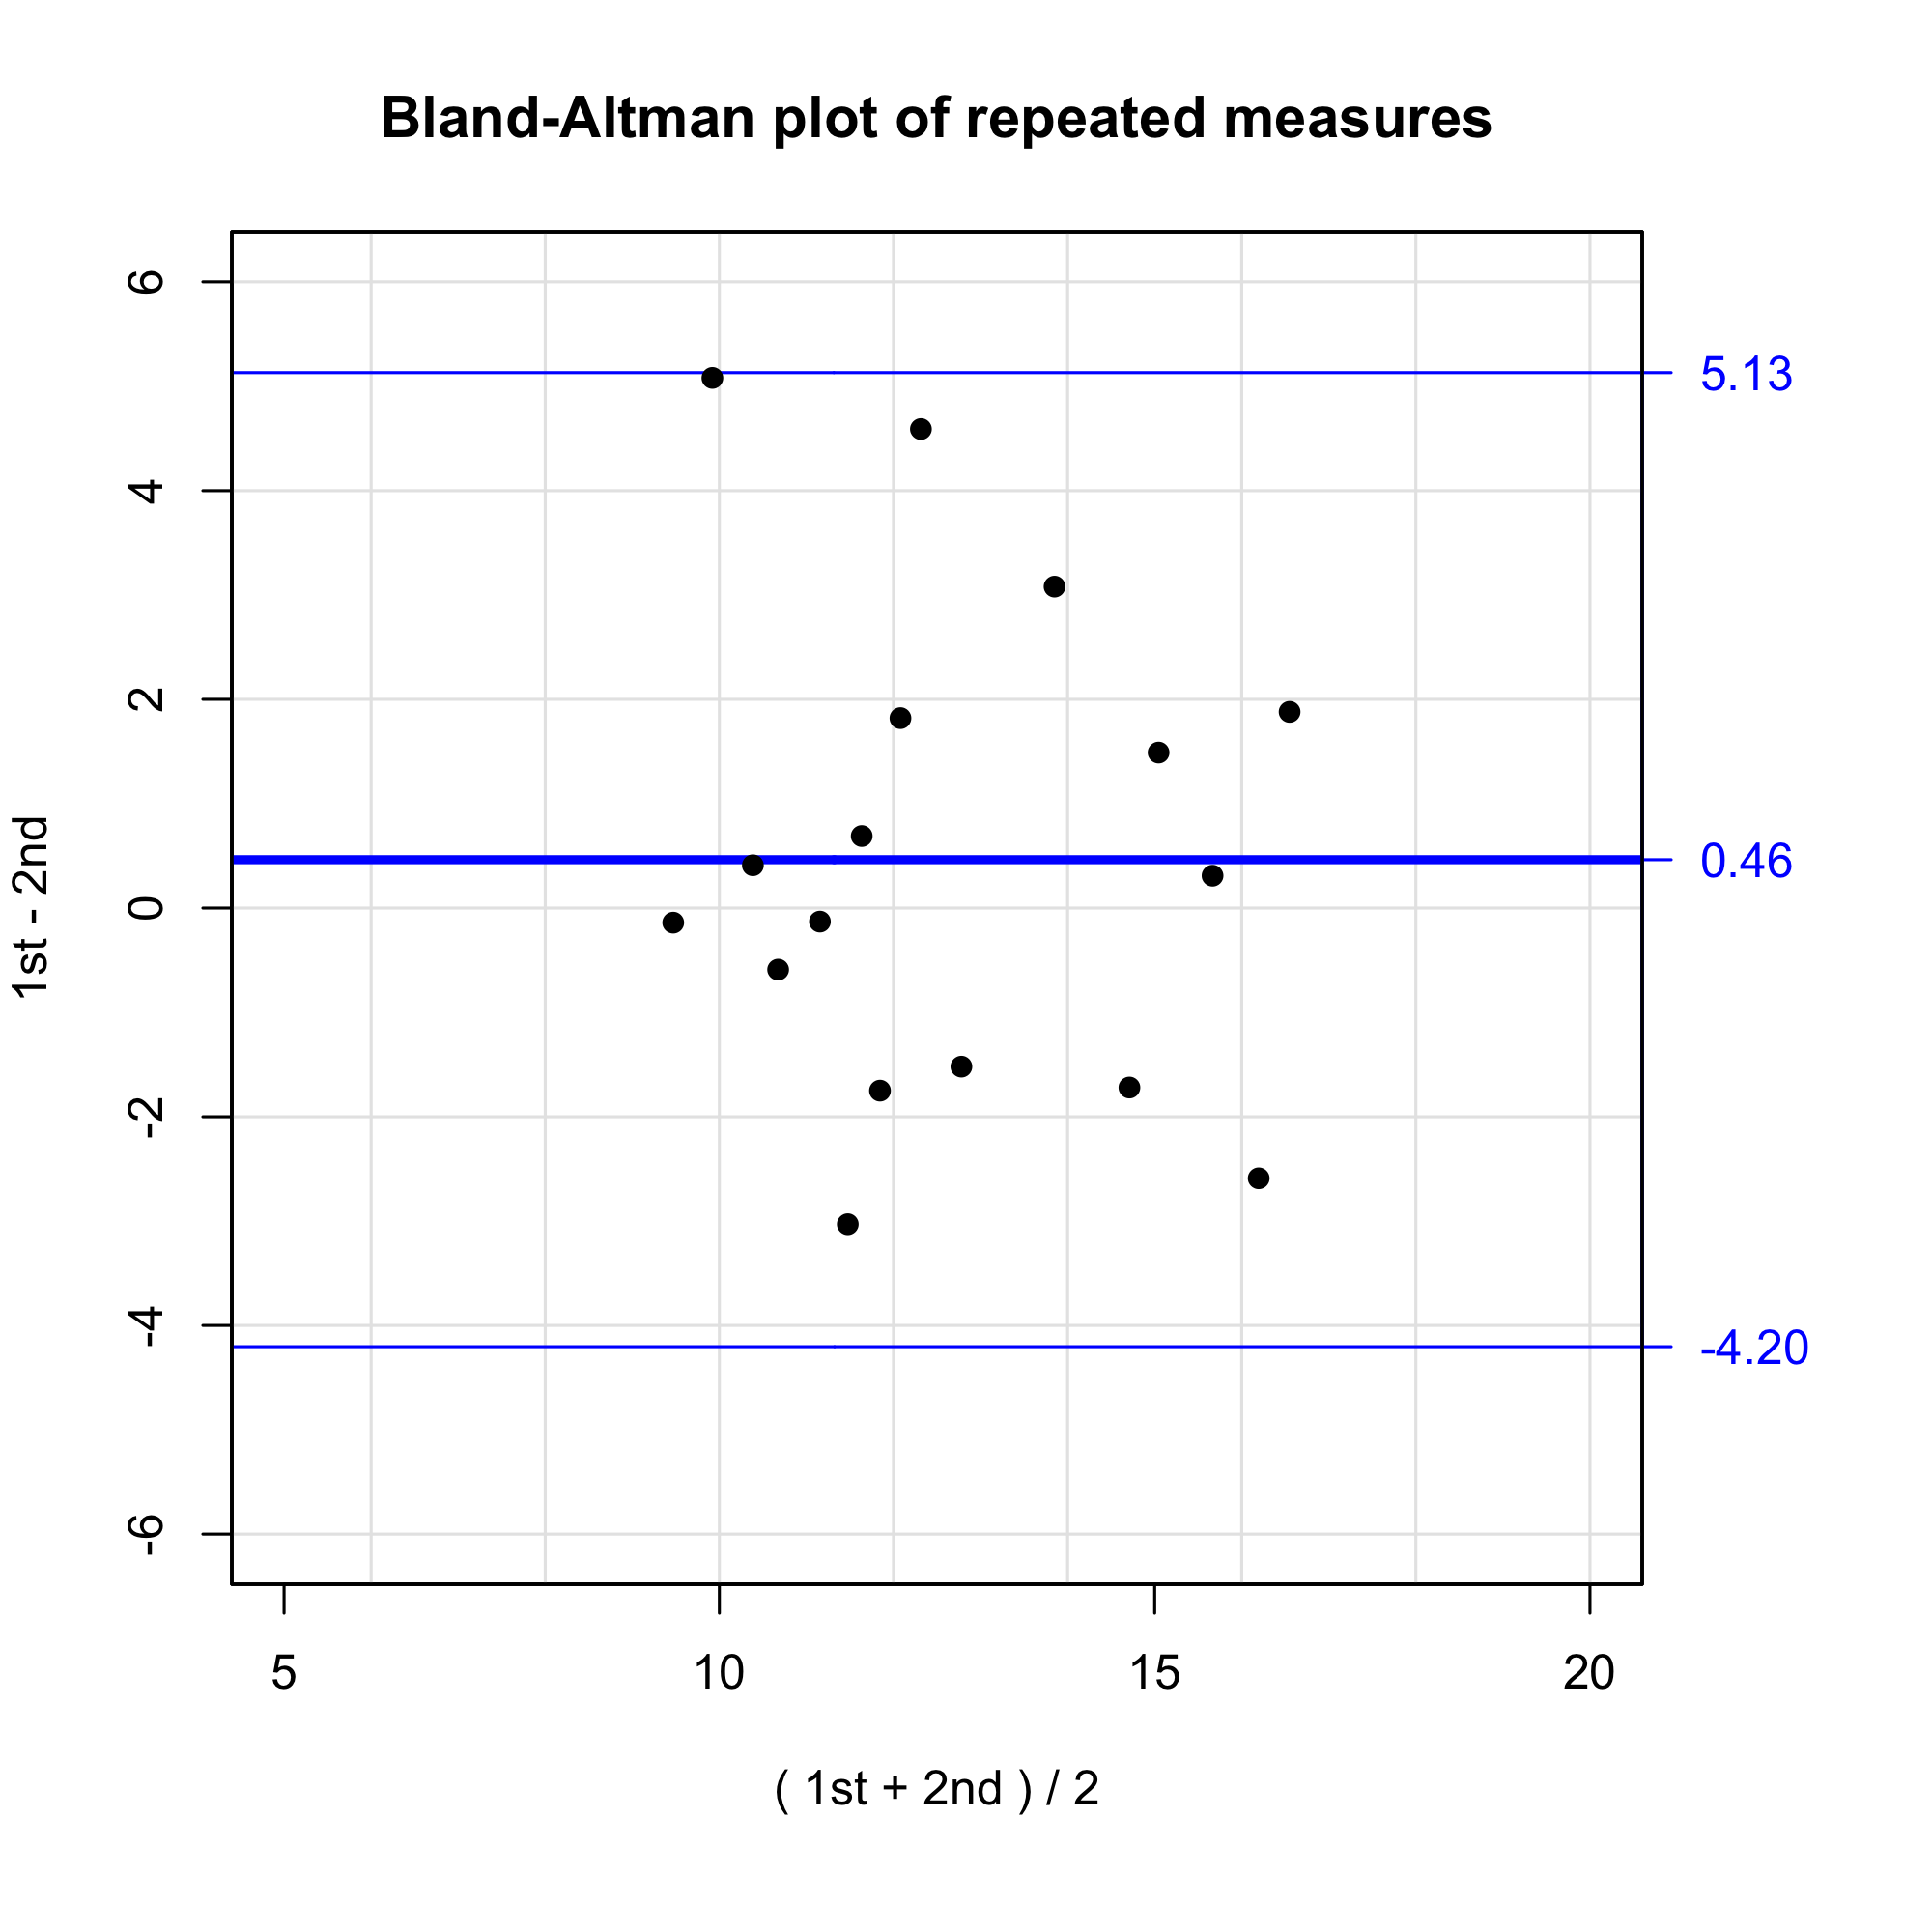
\includegraphics[scale=0.2]{ba_plot.png}
\caption{An example of Bland-Altman plot}
\end{center}
\end{figure}


\begin{table}[H]
\resizebox{1\textwidth}{!}{
\begin{minipage}{1\textwidth}
\begin{center}
\begin{tabular}{cccc}
\hline
 & $\Delta t=2$ & $\Delta t=4$ &$\Delta t=6$ \\
 \hline
& bias(lower, upper) & bias(lower, upper) & bias(lower, upper)\\
$t$=2 &	&	&\\
$t$=4 &	&	&\\
$t$=8 &	&	&\\
$t$=16 &	&	&\\
\hline
\end{tabular}
\label{tab:sim2}
\caption{Summary table of comparing the predictive results from proposed method with gold standard}
\end{center}
\end{minipage} 
}
\end{table}



% \section{Result}

% %%%%%%%%%%%%% insert table %%%%%%%%%%%%%%
% \small{
% \begin{center}
% \begin{sideways}
% \begin{tabular}{ccccccccccccccccccc}
% \hline
% \multicolumn{19}{c}{$\tau$=0.25}\\
% \hline
% &&&\multicolumn{2}{c}{${\beta_1}$}&\multicolumn{2}{c}{${\beta_2}$}&\multicolumn{2}{c}{${\delta_1}$}&\multicolumn{2}{c}{${\delta_2}$}&\multicolumn{2}{c}{${\gamma_1}$}&\multicolumn{2}{c}{${\gamma_2}$}&\multicolumn{2}{c}{$\alpha_1$}&\multicolumn{2}{c}{$\alpha_2$}\\
% n & $\alpha_1$ & $\alpha_2$ & bias & s.d. & bias & s.d.& bias & s.d.& bias & s.d.& bias & s.d. & bias & s.d. & bias & s.d. & bias & s.d. \\
% 250 & 0 & 0 & 0.05 & 0.108 & 0.00 & 0.106 & 0.02 & 0.108 & 0.00 & 0.131 & & & & & &&\\
% 250 & 1 & 0 & 0.077 & 0.119 & 0.011 & 0.111 & 0.001 & 0.094 & 0.037 & 0.096 & 0.033 & 0.078 & 0.003 & 0.077 & 0.014 & 0.109 & 0.024 & 0.190\\
% 250 & 0 & 1 & & & & & & & & & & & & & & & \\
% 250 & 1 & 1 & & & & & & & & & & & & & & & \\
% \hline
% \multicolumn{19}{c}{$\tau$=0.5}\\
% \hline
% &&&\multicolumn{2}{c}{${\beta_1}$}&\multicolumn{2}{c}{${\beta_2}$}&\multicolumn{2}{c}{${\delta_1}$}&\multicolumn{2}{c}{${\delta_2}$}&\multicolumn{2}{c}{${\gamma_1}$}&\multicolumn{2}{c}{${\gamma_2}$}&\multicolumn{2}{c}{$\alpha_1$}&\multicolumn{2}{c}{$\alpha_2$}\\
% n & $\alpha_1$ & $\alpha_2$ & bias & s.d. & bias & s.d.& bias & s.d.& bias & s.d.& bias & s.d. & bias & s.d. & bias & s.d. & bias & s.d. \\
% 250 & 0 & 0 & 0.05 & 0.108 & 0.00 & 0.106 & 0.02 & 0.108 & 0.00 & 0.131 & & & & & &&\\
% 250 & 1 & 0 & 0.077 & 0.119 & 0.011 & 0.111 & 0.001 & 0.094 & 0.037 & 0.096 & 0.033 & 0.078 & 0.003 & 0.077 & 0.014 & 0.109 & 0.024 & 0.190\\
% 250 & 0 & 1 & & & & & & & & & & & & & & & \\
% 250 & 1 & 1 & & & & & & & & & & & & & & & \\
% \hline
% \multicolumn{19}{c}{$\tau$=0.75}\\
% \hline
% &&&\multicolumn{2}{c}{${\beta_1}$}&\multicolumn{2}{c}{${\beta_2}$}&\multicolumn{2}{c}{${\delta_1}$}&\multicolumn{2}{c}{${\delta_2}$}&\multicolumn{2}{c}{${\gamma_1}$}&\multicolumn{2}{c}{${\gamma_2}$}&\multicolumn{2}{c}{$\alpha_1$}&\multicolumn{2}{c}{$\alpha_2$}\\
% n & $\alpha_1$ & $\alpha_2$ & bias & s.d. & bias & s.d.& bias & s.d.& bias & s.d.& bias & s.d. & bias & s.d. & bias & s.d. & bias & s.d. \\
% 250 & 0 & 0 & 0.05 & 0.108 & 0.00 & 0.106 & 0.02 & 0.108 & 0.00 & 0.131 & & & & & &&\\
% 250 & 1 & 0 & 0.077 & 0.119 & 0.011 & 0.111 & 0.001 & 0.094 & 0.037 & 0.096 & 0.033 & 0.078 & 0.003 & 0.077 & 0.014 & 0.109 & 0.024 & 0.190\\
% 250 & 0 & 1 & & & & & & & & & & & & & & & \\
% 250 & 1 & 1 & & & & & & & & & & & & & & & \\
% \hline
% % \captionof{table}{Caption.}
% % \label{tab:sim1}  
% \end{tabular}
% \end{sideways}
% \end{center}
% }












%%%%%%%%%%%%% insert figure %%%%%%%%%%%%%%
%\begin{figure}[H]
%\begin{center}
%\includegraphics[scale=0.2]{figure.jpg}
%\caption{An example figure.}
%\end{center}
%\end{figure}
%
%
%All is done in \LaTeX \cite{knuth1986texbook}.
%
%
% \bibliographystyle{plainnat}%%%%%%%%%%%%%%%%%%%%
% \addcontentsline{toc}{section}{References}
% \bibliography{QRJM}

% \end{document}